\documentclass[../../main.tex]{subfiles}
\begin{document}

\paragraph{【新課程】}
{\bf [解]}
$1$から$9$までの番号が書かれた$9$枚のカードを取り出す順序は全部で$9! = {}_9\mathrm{P}_9$通りあり，これらは同様に確からしい．
新しくつけられる番号が前もってつけられている番号に一致する$5$枚のカードの選び方は${}_9\mathrm{C}_5$通りある．
残りの$4$枚のカードについては，いずれも元の番号と異なる番号がつけられなければならない．
残る$4$枚のカードの元の番号を，一般性を失うことなく$1, 2, 3, 4$とする．
$1$のカードにつけられる新番号は$2, 3, 4$の$3$通りである．
ここで，$1$のカードに$2$の番号がつけられる場合を考えると，他の$3$枚（$2, 3, 4$）への番号の対応は以下の$3$通りである．
\begin{table}[h]
  \centering
  \begin{tabular}{|c|c|c|c|c|}
    \hline
    元の番号 & 1 & 2 & 3 & 4 \\ \hline
    新番号 (i) & 2 & 1 & 4 & 3 \\ \hline
    新番号 (ii) & 2 & 3 & 4 & 1 \\ \hline
    新番号 (iii) & 2 & 4 & 1 & 3 \\ \hline
  \end{tabular}
  \caption{残る$4$枚のカードの新番号の割り当て}
\end{table}
対称性より，$1$のカードに$3$，$4$の番号がつけられる場合も同様にそれぞれ$3$通りずつあるから，残る$4$枚のどのカードも元の番号と一致しない並べ方は
\begin{align}
  3 \times 3 = 9 \text{ 通り}
\end{align}
である．
したがって，一致するカードがちょうど$5$枚となる場合の数は
\begin{align}
  {}_9\mathrm{C}_5 \times 9 \text{ 通り}
\end{align}
である．ゆえに，求める確率$P$は
\begin{align}
  P &= \dfrac{{}_9\mathrm{C}_5 \times 9}{9!} \nonumber\\
  &= \dfrac{\dfrac{9!}{5! \, 4!} \times 9}{9!} \nonumber\\
  &= \dfrac{9}{5! \, 4!} \nonumber\\
  &= \dfrac{9}{120 \times 24} \nonumber\\
  &= \dfrac{1}{320} \tag{答}
\end{align}
である．

\paragraph{【旧課程】}
{\bf [解]}
自然数$n$に対し，線分$A_0A_n$の長さを$x_n$とおく．
条件より
\begin{align}
  x_1 = 1, \quad x_2 = 8
\end{align}
である．
$n \ge 3$に対して，点$A_{n-2}$，$A_{n-1}$のうち$A_0$に近い方を$X$，遠い方を$Y$とするから，
\begin{align}
  A_0X = \min(x_{n-2}, x_{n-1}), \quad A_0Y = \max(x_{n-2}, x_{n-1})
\end{align}
である．線分$A_0Y$を直径とする半円上に点$Z$があるから，$\angle A_0ZY = 90^\circ$である．
また，点$Z$から直径$A_0Y$（半直線$l$）に下ろした垂線の足が$X$であるから，直角三角形$\triangle A_0ZY$において
\begin{align}
  \triangle A_0XZ \sim \triangle A_0ZY
\end{align}
が成り立つ．

\begin{figure}[h]
  \centering
  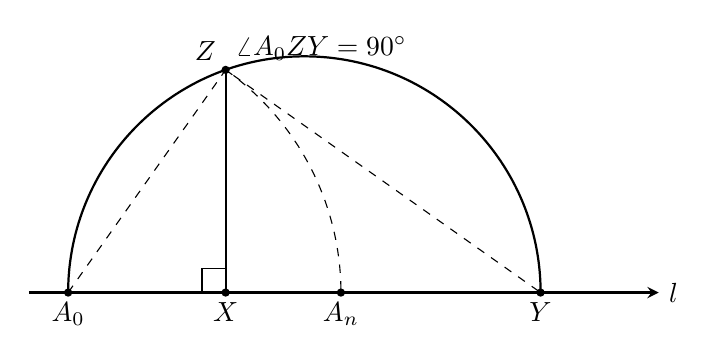
\begin{tikzpicture}[scale=1.0, >=stealth]
    \coordinate (A0) at (0,0);
    \coordinate (X) at (2,0);
    \coordinate (Y) at (6,0);
    \coordinate (Z) at (2, 2.828);
    \coordinate (An) at (3.464, 0);

    \draw[thick, ->] (-0.5,0) -- (7.5,0) node[right] {$l$};
    \draw[thick] (6,0) arc (0:180:3);
    \draw[dashed] (A0) -- (Z) -- (Y);
    \draw[thick] (X) -- (Z);
    \draw[dashed] (Z) arc (54.74:0:3.464);

    \draw (X) ++(0,0.3) -- ++(-0.3,0) -- ++(0,-0.3);

    \fill (A0) circle (1.5pt) node[below] {$A_0$};
    \fill (X) circle (1.5pt) node[below] {$X$};
    \fill (Y) circle (1.5pt) node[below] {$Y$};
    \fill (Z) circle (1.5pt) node[above left] {$Z$};
    \fill (An) circle (1.5pt) node[below] {$A_n$};

    \node[above right] at (Z) {$\angle A_0ZY = 90^\circ$};
  \end{tikzpicture}
  \caption{半円と垂線による点$Z$および点$A_n$の作図}
\end{figure}

相似比より
\begin{align}
  \dfrac{A_0X}{A_0Z} = \dfrac{A_0Z}{A_0Y} \Longleftrightarrow A_0Z^2 = A_0X \cdot A_0Y
\end{align}
である．$A_0X \cdot A_0Y = x_{n-2}x_{n-1}$であり，$A_0Z > 0$であるから，
\begin{align}
  A_0Z = \sqrt{x_{n-2}x_{n-1}}
\end{align}
となる．手順(2)より$x_n = A_0A_n = A_0Z$であるから，数列$\{x_n\}$の漸化式
\begin{align}
  x_n = \sqrt{x_{n-1}x_{n-2}} \quad (n \ge 3) \label{eq:1967-6old-rec}
\end{align}
を得る．
$x_1 = 1 > 0$，$x_2 = 8 > 0$より，すべての自然数$n$について$x_n > 0$である．
ここで両辺の$2$を底とする対数をとり，$y_n = \log_2 x_n$とおくと，
\begin{align}
  y_1 = \log_2 1 = 0, \quad y_2 = \log_2 8 = 3
\end{align}
であり，\eqref{eq:1967-6old-rec}より
\begin{align}
  y_n = \dfrac{y_{n-1} + y_{n-2}}{2} \quad (n \ge 3)
\end{align}
が成り立つ．変形すると
\begin{align}
  y_n - y_{n-1} = -\dfrac{1}{2}(y_{n-1} - y_{n-2}) \quad (n \ge 3)
\end{align}
となるから，数列$\{y_{n+1} - y_n\}$は初項$y_2 - y_1 = 3$，公比$-\dfrac{1}{2}$の等比数列である．
したがって，$n \ge 2$のとき
\begin{align}
  y_n - y_{n-1} = 3\left(-\dfrac{1}{2}\right)^{n-2}
\end{align}
である．これより，$n \ge 1$のとき（$n=1$でも成立）
\begin{align}
  y_n &= y_1 + \sum_{k=1}^{n-1} 3\left(-\dfrac{1}{2}\right)^{k-1} \nonumber\\
  &= 0 + 3 \cdot \dfrac{1 - \left(-\dfrac{1}{2}\right)^{n-1}}{1 - \left(-\dfrac{1}{2}\right)} \nonumber\\
  &= 2\left\{ 1 - \left(-\dfrac{1}{2}\right)^{n-1} \right\}
\end{align}
となる．
$n \to \infty$のとき$\left(-\dfrac{1}{2}\right)^{n-1} \to 0$であるから，
\begin{align}
  \lim_{n \to \infty} y_n = 2
\end{align}
である．$x_n = 2^{y_n}$であり，関数$f(t) = 2^t$は連続であるから，
\begin{align}
  \lim_{n \to \infty} x_n = 2^2 = 4
\end{align}
である．
したがって，点$A_n$が限りなく近づく定点を$A$とすると，線分$A_0A$の長さは
\begin{align}
  A_0A = 4 \tag{答}
\end{align}
である．

\end{document}
